\documentclass[a4paper,11pt]{article}
\usepackage{graphicx}
\usepackage[T1]{fontenc} % codifica dei font in uscita
\usepackage[utf8]{inputenc} % lettere accentate da tastiera
\usepackage[italian]{babel} % lingua principale del documento
\usepackage{url}
\usepackage [a4paper, top=2.5cm, bottom=2.5cm, left=1.5cm, right=1.5cm, bindingoffset=8mm] {geometry}

% inizio documento
             
\begin{document}

\begin{center}



\textsc{\Huge Esperienza V}\\[0.5cm]



\large
\title{ESPERIENZA IV}

Michele \textsc{Pedrotti}\\
Luigi \textsc{Bassini}\\
Nicola \textsc{Trevisson}\\


\end{center}
\vspace{0.1 cm}
\section{Scopo dell'esperienza}
 Lo scopo della nostra esperienza è la verifica della relazione empirica (legge di Lambert-Beer) che correla la quantità di luce assorbita da un mezzo alla natura chimica, alla concentrazione ed allo spessore del mezzo attraversato. La nostra esperienza, avendo a disposizione solamente il solfato di rame , si è svolta in due momenti: nella prima parte abbiamo variato la concentrazione della soluzione, mentre nella seconda abbiamo variato il cammino ottico (cioè lo spessore della soluzione attraversata).

\section{Verifica sperimentale della legge di Lambert-Beer}
\subsection{Relazione tra luce assorbita e concentrazione della soluzione}
Durante lo svolgersi dell'esperienza ci siamo serviti di una soluzione di solfato di rame a concentrazione molare 1 (e che consideriamo senza errore) messa a nostra disposizione. In seguito, grazie all'utilizzo di un cilindro graduato di risoluzione 1 ml, abbiamo diluito tale soluzione per ottenere diverse concentrazioni, grazie alla relazione: $$c\ped{1}\cdot V\ped{1}=c\ped{2}\cdot V\ped{2}$$ dove $c\ped{i}$ è la concentrazione, e $V\ped{i}$ rappresenta il volume della soluzione. La legge empirica che correla luce assorbita a concentrazione della soluzione e cammino ottico è: $$I\ped{m}=A\cdot e^{-k\cdot Lc}$$
dove $I\ped{m}$ è l'intensità luminosa espressa in W rilevata dopo che la radiazione elettromagnetica ha attraversato la cuvetta contenente la soluzione, c è la concentrazione della soluzione, k è l'assorbività specifica tipica del mezzo attraversato e L è il cammino ottico. La stessa legge può essere espressa nella forma: $$Y=a+bX$$ dove $X=log(I\ped{m})$, $a=log(A)$, $b=-kL$ e $X=c$.
Una volta ottenute diverse concentrazioni, abbiamo misurato l'intensità luminosa in uscita, e rappresentato in grafico i dati sperimentali ottenuti:   

 \begin{center} 
\begin{figure}[htpd]
\hspace{0 pt}
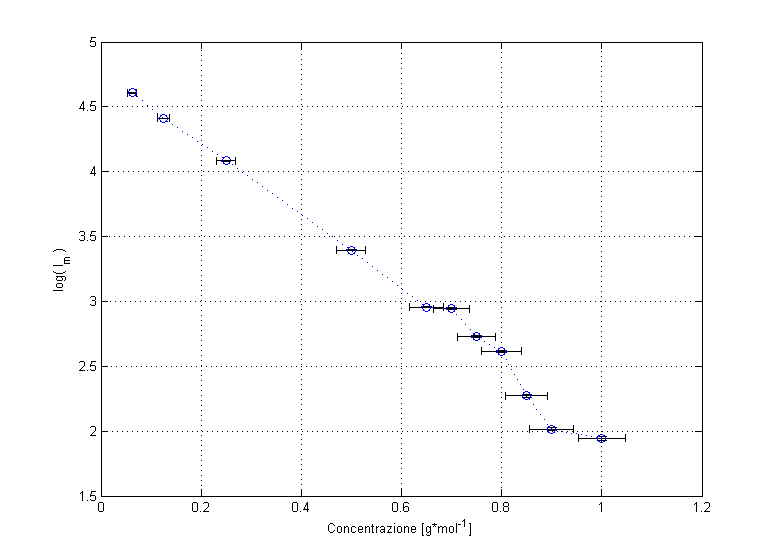
\includegraphics[scale=0.80]{grafico1.png}


\end{figure}
\end{center}
\vspace{7 cm}
Possiamo notare che i dati relativi a concentrazioni vicine a 1 non seguono un andamento perfettamente lineare. Questo può essere spiegato considerando le difficoltà pratiche dell'esperimento: per ottenere soluzioni di queste concentrazioni infatti è necessario aggiungere quantità esigue di acqua. Tramite regressione lineare abbiamo calcolato i parametri del fit, e tramite questi abbiamo potuto calcolare A e k, ottenendo i seguenti risultati: $A = 118  \pm 1 \mu W $,$k = 2.51 \pm 0.01 mol\cdot g^{-1}$. Notiamo inoltre che la concentrazione 0 non corrisponde all'intensità del laser se il mezzo attraversato fosse l'aria. Bensì se la concenrazione fosse 0 il mezzo attraversato sarebbe l'acqua. Confrontando il valore di A da noi trovato e il valore $I\ped m$ corrispondente all'acqua ($116  \pm 1 \mu W $) possiamo affermare la compatibilità tra i due valori.   


\subsection{Relazione tra luce assorbita e cammino ottico}
A differenza del caso precedente durante questa parte dell'esperienza si è mantenuta costante la concentrazione (pari a 0.125 $g\cdot mol^{-1}$) mentre si è variato il cammino ottico medio.
Questo ci ha permesso di verificare come con l'aumentare del cammino ottico medio la luce assorbita dalla soluzione aumenti in maniera lineare.
I dati ottenuti sono riportati nel seguente grafico.
\vspace{2000 pt}
 \begin{center} 
\begin{figure}[htpd]
\hspace{0 pt}
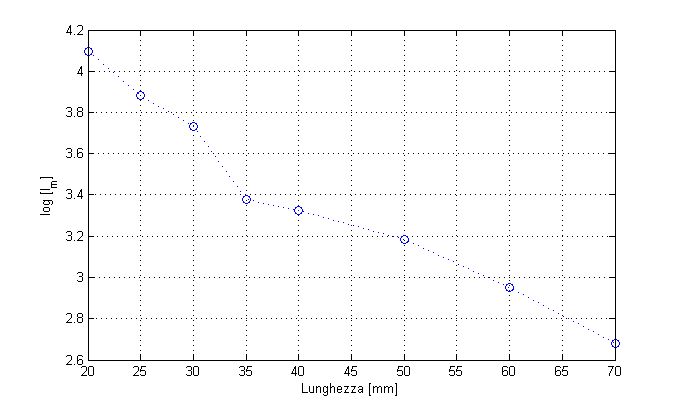
\includegraphics[scale=0.80]{grafico2.png}
\end{figure}
\end{center}
Si può notare come i dati tendano a seguire un andamento lineare
Utilizzando ancora la legge : $$I\ped{m}=A\cdot e^{-k\cdot Lc}$$
che può essere espressa nella forma: $$Y=a+bX$$ dove $X=log(I\ped{m})$, $a=log(A)$, $b=-k$ e $X=cL$. 
Tramite la regressione lineare abbiamo calcolato i parametri del fit con i quali abbiamo potuto calcolare A e k con i seguenti risultati:
 $A = 109  \pm 4 \mu W $,$k = 2.7 \pm 0.1 mol\cdot g^{-1}$.
 Possiamo notare che i valori di A e di k non sono compatibili con quelli calcolati nella prima parte dell'esperienza. Bisogna altrsì notare che la concentrazione utilizzata per la seconda parte dell'esperienza è stata ottenuta mischiando insieme la soluzione a concentrazione 0.125 ottenuta da tutti i gruppi di laboratorio. E' quindi plausibile ammettere una variazione importante della concentrazione rispetto alla concentrazione supposta. Invertendo la formula e supponendo un k pari a quello calcolato nella prima parte dell'esperienza otteniamo un valore della soluzione pari a $0.132 g*mol^{-1}$. Per quanto detto fino ad ora consideriamo tale valore plausibile, e consideriamo i valori trovati nella prima e nella seconda parte dell'esperienza compatibili tra loro.
 






\end{document}